\documentclass[12pt]{article}
\usepackage[letterpaper, margin=1in]{geometry}
\usepackage{graphicx}
\usepackage{amsmath}
\usepackage[framed, numbered]{matlab-prettifier}
\lstset{inputpath=../Matlab}
\graphicspath{{../Figures/}}
\title{ELECENG 3TP3 Lab 2}
\author{Raeed Hassan \\ hassam41 \\ McMaster University}
\begin{document}
\maketitle
\pagebreak
\begin{enumerate}
    \item 
    Part a)
    \begin{enumerate}
        \item
        \begin{equation*}
        \begin{aligned}
            x[i] &= [1,1,1],\; v[i] = [1,1,1,1] \\
            y[n] &= \sum_{i=-\infty}^{\infty} \; x[i] \, v[n-i] \\
            y[0] &= x[0] \, v[0] = 1\cdot1 = 1 \\
            y[1] &= x[0] \, v[1] + x[1] \, v[0] = 1 + 1 = 2 \\
            y[2] &= x[0] \, v[2] + x[1] \, v[1] + x[2] \, v[0] = 3 \\
            y[3] &= x[0] \, v[3] + x[1] \, v[2] + x[2] \, v[1] = 3 \\
            y[4] &= x[1] \, v[3] + x[2] \, v[2] = 2 \\
            y[5] &= x[2] \, v[3] = 1 \\
            y[6] &= 0 \\
            y[n] &= \begin{cases}
                1, & n=0,5 \\
                2, & n=1,4 \\
                3, & n=2,3 \\
                0, & \text{otherwise}
            \end{cases}
        \end{aligned}
        \end{equation*}
        \item
        \begin{equation*}
            \begin{aligned}
                x[i] &= [2,1],\; v[i] = [1,1,1,1] \\
                y[n] &= \sum_{i=-\infty}^{\infty} \; x[i] \, v[n-i] \\
                y[0] &= x[0] \, v[0] = 2 \\
                y[1] &= x[0] \, v[1] + x[1] \, v[0] = 2 + 1 = 3 \\
                y[2] &= x[0] \, v[2] + x[1] \, v[1] = 3 \\
                y[3] &= x[0] \, v[3] + x[1] \, v[2] = 3 \\
                y[4] &= x[1] \, v[3] = 1 \\
                y[5] &= 0 \\
                y[n] &= \begin{cases}
                    1, & n=4 \\
                    2, & n=0 \\
                    3, & n=1,2,3 \\
                    0, & \text{otherwise}
                \end{cases}
            \end{aligned}
        \end{equation*}
        \item
        \begin{equation*}
            \begin{aligned}
                x[i] &= [2,1],\; v[i] = [0,1,2] \\
                y[n] &= \sum_{i=-\infty}^{\infty} \; x[i] \, v[n-i] \\
                y[0] &= x[0] \, v[0] = 2\cdot0 = 0 \\
                y[1] &= x[0] \, v[1] + x[1] \, v[0] = 2 \\
                y[2] &= x[0] \, v[2] + x[1] \, v[1] = 5 \\
                y[3] &= x[1] \, v[2] = 2 \\
                y[4] &=  0 \\
                y[n] &= \begin{cases}
                    2, & n=1,3 \\
                    5, & n=2 \\
                    0, & \text{otherwise}
                \end{cases}
            \end{aligned}
        \end{equation*}
    \end{enumerate}
    Part b)

    The MATLAB code used to verify these results is shown in Listing \ref{listing:part1b}. The script simply assigns the data for each signal into an array, and calculates the convolution of each pair of $x[n]$ and $v[n]$.
    \lstinputlisting[style=Matlab-editor, caption={Part 1b}, label={listing:part1b},lastline=6]{question1b.m}
    The MATLAB code used to plot and export the stem plots is shown in Listing \ref{listing:part1b_plots}. The portion of the script creates subplots for each plot, then plots a stem plot into the subplot. Each stem plot has been given appropriate axis limits for viewing the data. The plots are shown in Figure \ref{fig:part1b_plots}.
    \lstinputlisting[style=Matlab-editor, caption={Part 1b stem plots}, label={listing:part1b_plots},firstnumber=8,firstline=8]{question1b.m}
    \begin{figure}[ht]
        \centering
        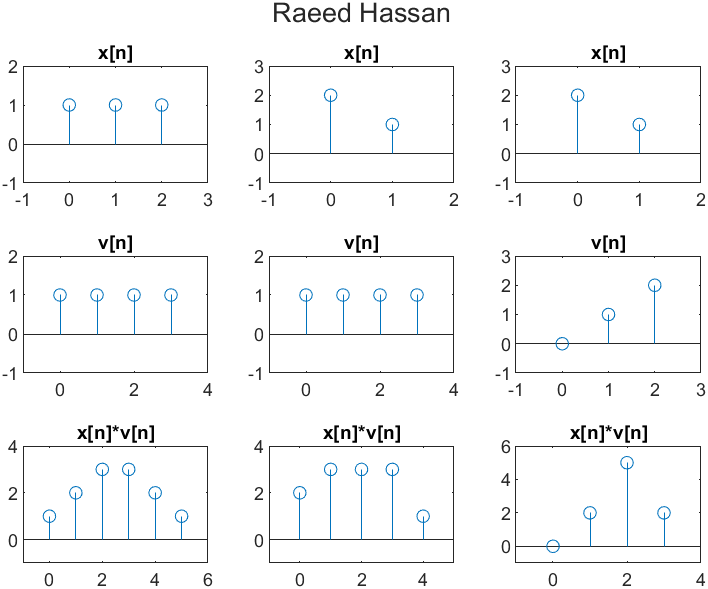
\includegraphics[width=0.97\textwidth]{question1b.png}
        \caption{\label{fig:part1b_plots}Part 1b Plots}
    \end{figure}
    \setcounter{enumi}{3}
    
    \item 
    The MATLAB code used to generated the distorted signal is shown in Listing \ref{listing:part4}. The script calls the MATLAB code described in part 3 to read the \verb|speech.wav| audio file. The script calculates the echo delay, \verb|Te|, in seconds and stores this value in \verb|Te_sec|. The number of sample points on the original signal that the echo would be delayed by is calculated by dividing the echo delay in seconds, \verb|Te_sec|, by the sampling period of the original signal, \verb|T|, and stored in the variable \verb|L_delay|. The value of \verb|L_delay| is rounded to ensure that the sample delay is always an integer.

    The signal \verb|signalplusecho| is initialized as a column vector of size \verb|L+L_delay| filled with 0s. The start of the new signal is set to the original signal. The amplified echo signal is added to the new signal at appropriately shifted indices. The new signal was re-scaled to ensure the signal does not clip, then written to a new wav file \verb|speechwithecho.wav|.

    \lstinputlisting[style=Matlab-editor, caption={Part 4}, label={listing:part4}]{question4.m}
    
    \item
    The MATLAB code used to generated the distorted signal using convolution is shown in Listing \ref{listing:part5}. The script calculates the number of samples the echo is delayed by. The impulse response, \verb|IR|, was simply chosen to be the starting samples for the original signal and the echo. A column vector filled with 0s of size \verb|L_delay|+1 was created, and the impulses for the original signal (value of 1) and the echo (value of reduced amplitude factor, $\alpha$) were assigned at indices 1 and \verb|L_delay|+1. The distorted signal, \verb|signalplusecho_conv|, was determined by calculating the convolution of the original signal and the impulse response. The distorted signal was re-scaled to ensure the signal does not clip, then written to a new wav file \verb|speechwithecho_conv.wav|. 

    \lstinputlisting[style=Matlab-editor, caption={Part 5}, label={listing:part5}]{question5.m}

    \item
    When the value of \verb|alpha| is equal to 1, the value of \verb|Te| must be around 120 ms before the quality of speech is acceptable. At higher values of \verb|Te|, it is either difficult to identify that there is only one signal that is supposed to be transmitted, or the echo interferes with the receiver's ability to clearly understand the original signal. At values of \verb|Te| less than 120 ms, the receiver can both identify that there is a single signal that was intended to be transmitted and understand the contents of the signal relatively clearly.

    The value of \verb|Te| for the quality of the speech to be acceptable does not change from 120 ms as the value of \verb|alpha| decreases, until the value of \verb|alpha| is sufficiently low that the receiver can tune out the echo (\verb|alpha| $\approx$ 0.05). The echo can still be interpreted as a second signal and interfere with the user's ability to clearly understand the contents of the original signal, even while adjusting the value of \verb|Te|. It is only when the echo is quiet enough the user can largely ignore it, can the value of \verb|Te| be increased to any value with the quality of speech remaining acceptable.

    \item
    The MATLAB code used to generated the distorted signal using convolution is shown in Listing \ref{listing:part7}. The MATLAB script is very similar to the one used for part 5, with the only differences being an additional variable \verb|num_echos| to store the number of echos, and the impulse response \verb|IR| being generated differently. The size of \verb|IR| is \verb|num_echos*L_delay|+1 instead of \verb|L_delay|+1 as there are multiple additional echos that have to be accounted for at the end of the signal. The exponentially decaying impulses are added to the impulse response using a for loop. The convolution of the  original signal and impulse response is calculated and stored in \verb|signalplusreverb|.  The distorted signal was re-scaled to ensure the signal does not clip, then written to a new wav file \verb|speechwithreverb.wav|. 

    \lstinputlisting[style=Matlab-editor, caption={Part 7}, label={listing:part7}]{question7.m}

    When the value of $N_e$ was equal to 1, the signal was identical to the signal examined in part 6, and the observations about \verb|alpha| and \verb|Te| remain the same.

    When the value of $N_e$ increased and the value of \verb|alpha| was 1, the value of \verb|Te| to make the quality of speech acceptable depended on the value of $N_e$. As the value of $N_e$ increases, the value of \verb|Te| required to make the quality of speech acceptable decreases. It was observed that the quality of speech remained acceptable as long as the delay between the last echo and the original signal remained around the 120 ms value (\verb|Te| $\times$ \verb|num_echos| $\approx$ 120 ms) observed in part 6. This was observed with values of $N_e$ as high as 1000. As you increased the delay above the 120 ms delay, the quality of speech sharply degraded as you would begin to hear multiple distinct speeches or high-pitched noise in the signal.
    
    When the value of $N_e$ increased and the value of \verb|alpha| was decreased, the value of \verb|Te| or $N_e$ do not change until the value of \verb|alpha| is sufficiently low that the receiver can tune out all the echos (\verb|alpha| $\approx$ 0.05), similarly to what was observed in part 6. The echo can still be interpreted as a second signal and interfere with the user's ability to clearly understand the contents of the original signal, even while adjusting the values of \verb|Te| and \verb|num_echos|. The value of \verb|Te| $\times$ \verb|num_echos| needed to keep the quality of speech acceptable remains at around 120 ms, until the value of \verb|alpha| is low enough the user can ignore the echos. At values of \verb|alpha| lower than this point, the values of \verb|Te| and \verb|num_echos| can be changed freely without having a significant effect on the quality of speech.
\end{enumerate}
\end{document}